\documentclass[usenames,dvipsnames,notes]{beamer}
\usepackage{ifthen}
\usepackage{xcolor}
\usepackage{pgfplots}
\usepackage{amsmath}
\usepackage{centernot}
\usepackage{pifont}
\usepackage{tabularx}
\usepackage{makecell}
\usepackage{cuted}
\usepackage{booktabs}
\usepackage{array}
\usepackage{caption}
\usepackage{subcaption}

\usepackage{pgfpages}
%\setbeameroption{show notes on second screen}


\input ../beamer-style
\input ../std-macros
\input ../macros

\AtBeginSection[]
{
    \begin{frame}
        \frametitle{Table of Contents}
        \tableofcontents[currentsection]
    \end{frame}
}
\parskip=10pt

\title[CSCI-GA.2590]{Context-Free Parsing}
\author[He He]{He He
}
\institute[NYU]{New York University}
\date{\today}

\begin{document}
\begin{frame}
\titlepage
\end{frame}

\begin{frame}
    {Logistics}
    \begin{itemize}
        \item Homework 3
        \item Project proposal and group
        \item Project presentation
    \end{itemize}
\end{frame}

\section{Context-free language}

\begin{frame}
    {Langauge is a set of strings}
    \textbf{Formal language}:\\
    \begin{itemize}
        \item A set of \textbf{strings} consisting of \textbf{words} from an \textbf{alphabet}
        \item \emph{Well-formed} according to a set of rules 
        \item Studies the \emph{syntactical} aspects of a language
    \end{itemize}

    Examples:\\
    \begin{itemize}
        \item Formulas (logic): $(p_1 \wedge p_2) \vee (\urcorner p_3)$
        \item Programming languages: \texttt{int a, b = 0;}
        \item Sequences from the alphabet $\pc{a,b}$ that ends with two $a$'s
    \end{itemize}

    Questions:\\
    \begin{itemize}
        \item Formal language theory: expressiveness power, recognizability etc.
        \item Can we design formal languages that capture as many properties of natural language as possible? 
    \end{itemize}
\end{frame}

\begin{frame}
    {Context-free language}
    \textbf{Context-free languages (CFL)} are generated by a \textbf{context-free grammar} $G=(\Sigma, N, R, S)$:\\
    \begin{itemize}
        \item a finite alphabet $\Sigma$ of \textbf{terminals} (words)
        \item a finite set of \textbf{non-terminals} $N$ disjoint from $\Sigma$ (word groups)
        \item a set of \textbf{production rules} $R$ of the form $A\rightarrow\beta$,
            where $A \in N, \beta \in (\Sigma \cup N)^*$ (how to group words)
        \item a start symbol $S\in N$ (root of derivation)
    \end{itemize}

    Example:\\
    \begin{itemize}
        \item[] $S\rightarrow SS$
        \item[] $S\rightarrow (S)$
        \item[] $S\rightarrow ()$
    \end{itemize}
\end{frame}

\begin{frame}
    {Natural language syntax}
    Construct a formal language to represent the syntax of natural language\\
    \begin{itemize}
        \item \emph{Expressivity}: how many syntactic phenomena can it cover?
        \item \emph{Computation}: how fast can we parse a sentence?
    \end{itemize}

    Context-free grammars for natural language\\
    \begin{itemize}
        \item Captures nested structures which are common in natural language 
            \begin{itemize}
                \item[] [I told Mary that [John told Jane that [Ted told Tom a secret]]].
            \end{itemize}
        \item Captures long-range dependencies
            \begin{itemize}
                \item[] \emph{the} burnt and badly-ground Italian \emph{coffee}
                \item[] \emph{these} burnt and badly-ground Italian \emph{coffees}
            \end{itemize}
        \item Strikes a good balance between expressivity and computation
    \end{itemize}
\end{frame}

\begin{frame}
    {Phrase-structure grammar for English}
    Sentences are broken down into \textbf{constituents}.

    A constituent works as a single unit in a sentence.\\
    \begin{itemize}
        \item Can be moved around or replaced without breaking grammaticality.
        \item[] (Abigail) and (her younger brother) (bought a fish).
    \end{itemize}

    Construct CFG for English\\
    \begin{itemize}
        \item Each word is a terminal, derived from its POS tag.
        \item Each sentence is derived from the start symbol $S$.
        \item Each phrase type is a non-terminal.
        \item Each constituent is derived from a non-terminal.
    \end{itemize}

    Grammar design: choose the right set of non-terminals that produces different constituents.
\end{frame}

\begin{frame}
    {A toy example CFG}
    \begin{figure}    
        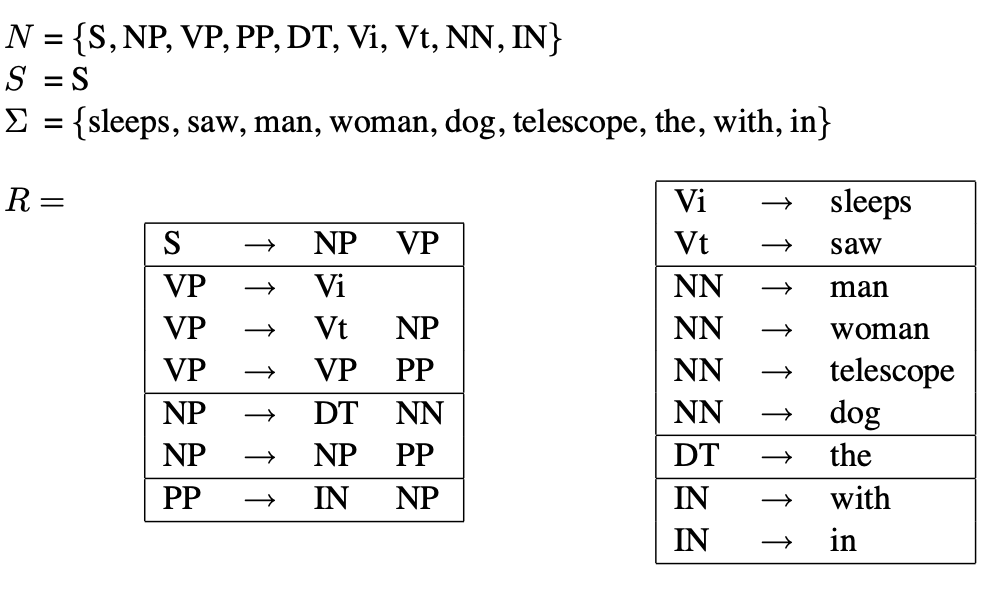
\includegraphics[height=6cm]{figures/toy-cfg.png}
    \end{figure}   
    \vspace{-2em}
    \textbf{Lexicon}: rules that produce the terminals
\end{frame}

\begin{frame}
    {Parsing}
    \begin{figure}    
        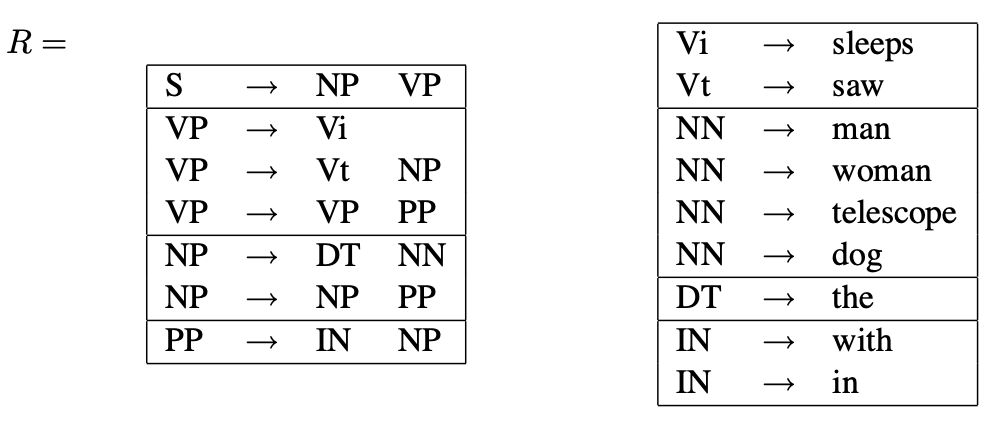
\includegraphics[height=4cm]{figures/toy-cfg-2.png}
    \end{figure}  
    \vspace{-2em}
    Can we derive the sentence ``the man sleeps''?
    \vspace{9em}
\end{frame}

\begin{frame}
    {Ambiguity}
    Can a sentence have multiple parse trees?
    \begin{figure}
        \begin{subfigure}[b]{0.45\textwidth}
            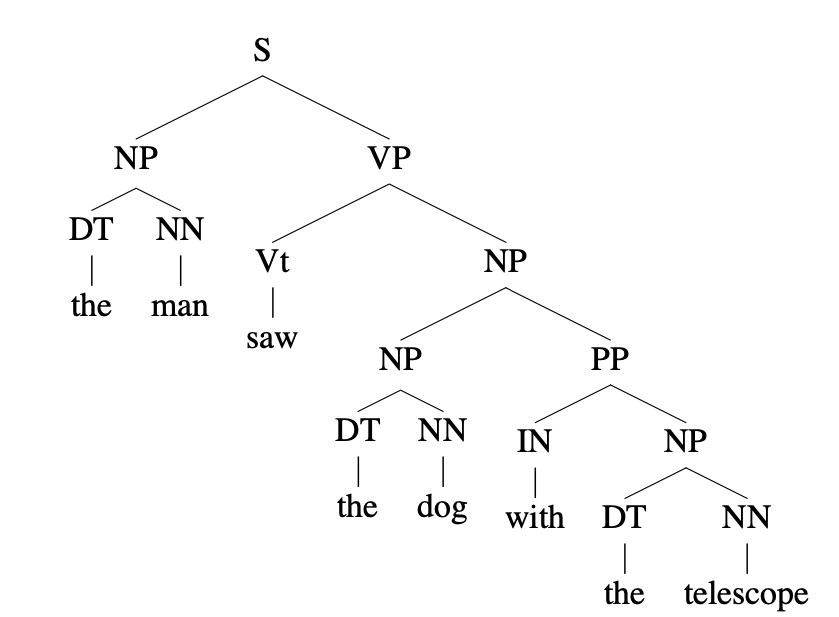
\includegraphics[width=\textwidth]{figures/parse-1.png}
        \end{subfigure}
        \begin{subfigure}[b]{0.45\textwidth}
            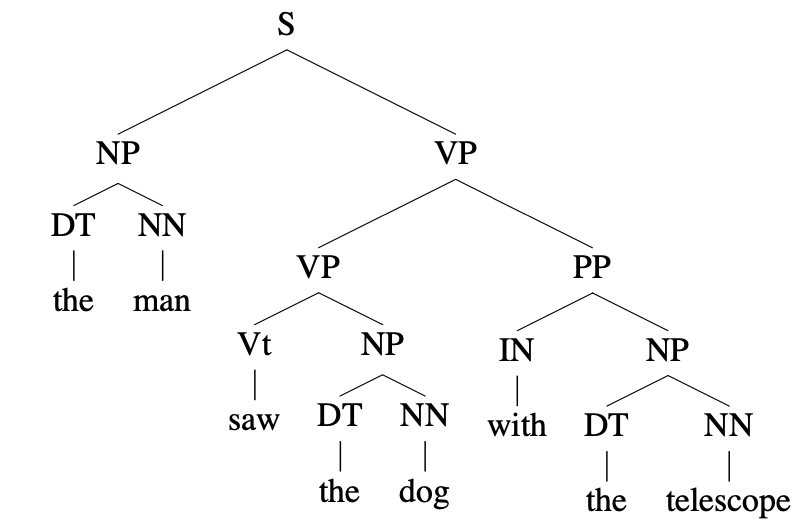
\includegraphics[width=\textwidth]{figures/parse-2.png}
        \end{subfigure}
    \end{figure}

    Exercise: find parse trees for\\
    ``She announced a program to promote safety in trucks and vans''.
\end{frame}

\section{Probabilistic context-free grammars}

\begin{frame}
    {PCFG}
    Notation: let $\sT_G$ be the set of all possible left-most parse trees under the grammar $G$.

    Goal: define a probability distribution $p(t)$ over parse trees $t\in\sT_G$

    Parsing: pick the most likely parse tree for a sentence $s$
    $$
    \argmax_{t\in\sT_G(s)} p(t)
    $$

    Three questions:\\
    \begin{itemize}
        \item Modeling: how to define $p(t)$ for trees?
        \item Learning: how to estimate parameters of the distribution $p(t)$?
        \item Inference: how to find the most likely tree efficiently?
    \end{itemize}
\end{frame}

\begin{frame}
    {Modeling}
    Generate parse trees: iteratively sample a production rule to expand a non-terminal
    \vspace{-1em}
    \begin{figure}    
        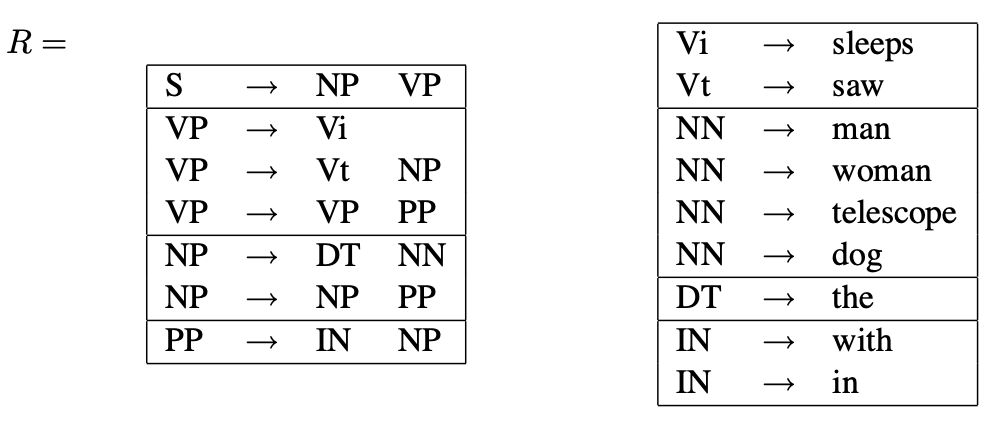
\includegraphics[height=4cm]{figures/toy-cfg-2.png}
    \end{figure}  
    \vspace{7em}
\end{frame}

\begin{frame}
    {PCFG}
    A \textbf{PCFG} consists of\\
    \begin{itemize}
        \item A CFG $G=(\Sigma, N, R, S)$
        \item Probabilities of production rules $q(\alpha\rightarrow\beta)$ for each $\alpha\rightarrow\beta\in R$ such that
            $$
            \sum_{\beta\colon X\rightarrow\beta\in R}q(X\rightarrow\beta) = 1
            \quad \forall X\in N
            $$
    \end{itemize}
    \vspace{-1em}
    \begin{figure}    
        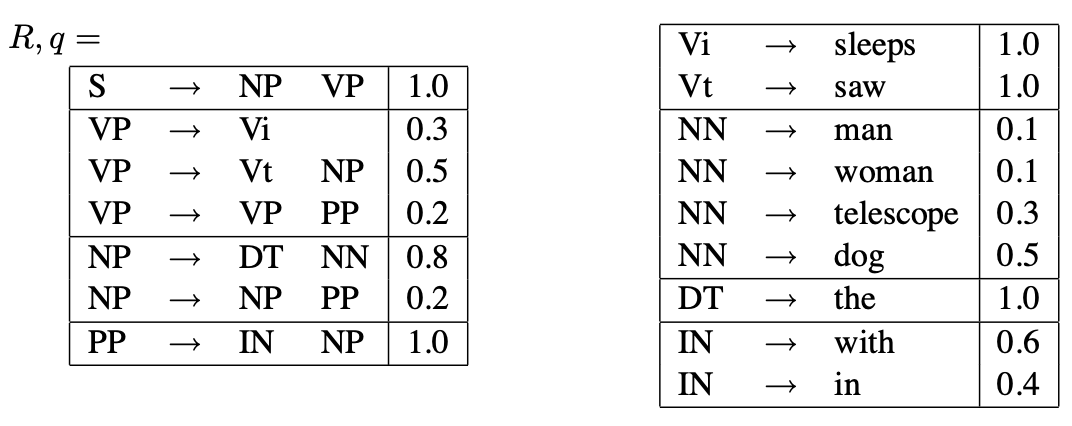
\includegraphics[height=4cm]{figures/toy-pcfg.png}
    \end{figure}  
\end{frame}

\begin{frame}
    {From HMM to PCFG}
\end{frame}

\begin{frame}
    {Probabilities of parse trees}
    Given a parse tree $t$ consisting of rules
    $\alpha_1\rightarrow\beta_1,\ldots, \alpha_n\rightarrow\beta_n$,
    its probabilities under the PCFG is
    $$
    p(t) = \prod_{i=1}^n q(\alpha_i\rightarrow\beta_i)
    $$
    \vspace{-1em}
    Example:

    \begin{columns}
        \begin{column}{0.5\textwidth}
    \begin{figure}    
        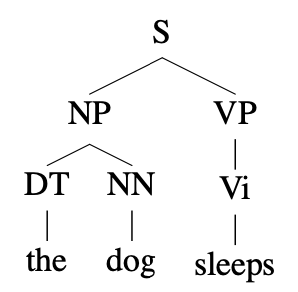
\includegraphics[height=3cm]{figures/toy-tree.png}
    \end{figure}  
        \end{column}
        \begin{column}{0.5\textwidth}
        \end{column}
    \end{columns}
\end{frame}

\begin{frame}
    {Learning}
    Given a set of trees,
    we can estimate rule probabilities by MLE.
    \pause
    $$
    q(\alpha\rightarrow\beta) = \frac{\text{count}(\alpha\rightarrow\beta)}{\sum_{\beta'\colon\alpha\rightarrow\beta'\in R}\text{count}(\alpha\rightarrow\beta')}
    $$
    Training data: treebanks
    \vspace{-1em}
    \begin{figure}    
        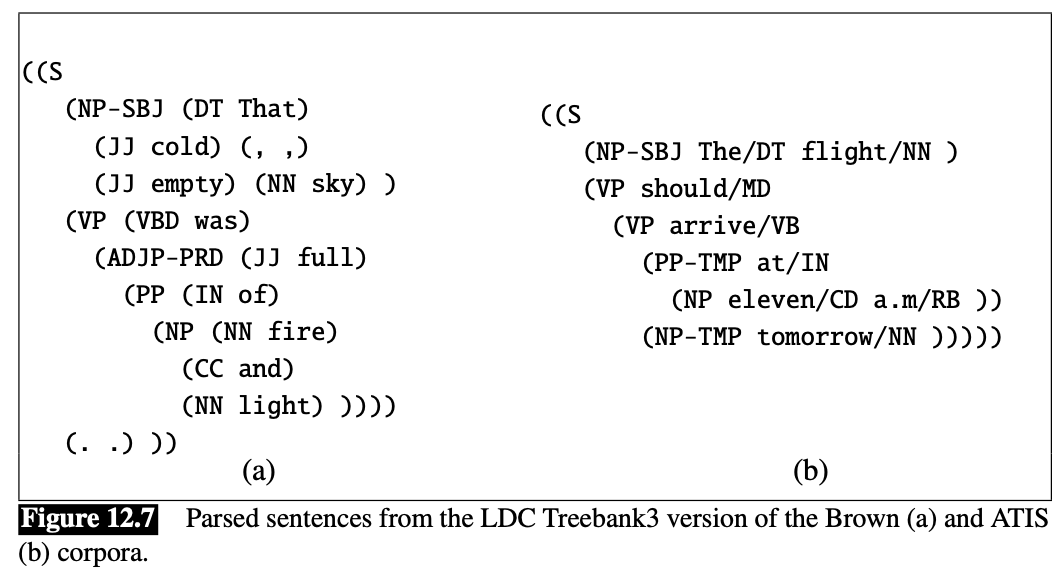
\includegraphics[height=4cm]{figures/treebank.png}
    \end{figure}  
\end{frame}

\begin{frame}
    {Parsing}
    Input: sentences, (P)CFG \\
    Output: derivations / parse trees (with scores/probabilities)

    Total number of parse trees for a sentence?

    Consider a minimal CFG:\\
    \begin{itemize}
        \item[] $X\rightarrow XX$
        \item[] $X\rightarrow \text{aardvark} | \text{abacus} | \ldots | \text{zyther}$
    \end{itemize}

    \# of parse trees = \# of strings with balanced brackets\\
    \begin{itemize}
        \item[] $((w_1 w_2) (w_3 w_4))$, $(((w_1 w_2) w_3) w_4)$, ...
    \end{itemize}

    \# of strings with $n$ pairs of brackets:
    $$
    \text{Catalan number } C_n = \frac{1}{n+1}{2n\choose n}
    $$
\end{frame}

\begin{frame}
    {Chomsky normal form (CNF)}
    A CFG is in \textbf{Chomsky normal form} if every production rule takes one of the following forms:
    \begin{itemize}
        \item Binary non-terminal production: $A\rightarrow BC$ where $A, B, C\in N$.
        \item Unary terminal production: $A\rightarrow a$ where $A\in N, a\in\Sigma$.
    \end{itemize}

    Grammars in CNF produces \emph{binary} parse trees.

    Convert a production rule to CNF: VP $\rightarrow$ VBD NP PP\\
    \begin{itemize}
        \item[] VP $\rightarrow$ VBD @VP-VBD
        \item[] @VP-VBD $\rightarrow$ NP PP
    \end{itemize}

    We assume the grammar are in CNF.
\end{frame}

\begin{frame}
    {Dynamic programming on the tree}
    $$
    p(t) = \underbrace{q(A\rightarrow B C)}_{\text{top rule}}
    \times \underbrace{q(t_B)}_{\text{left child}}
    \times \underbrace{q(t_C)}_{\text{right child}}
    $$
    \vspace{-1em}
    \begin{figure}
        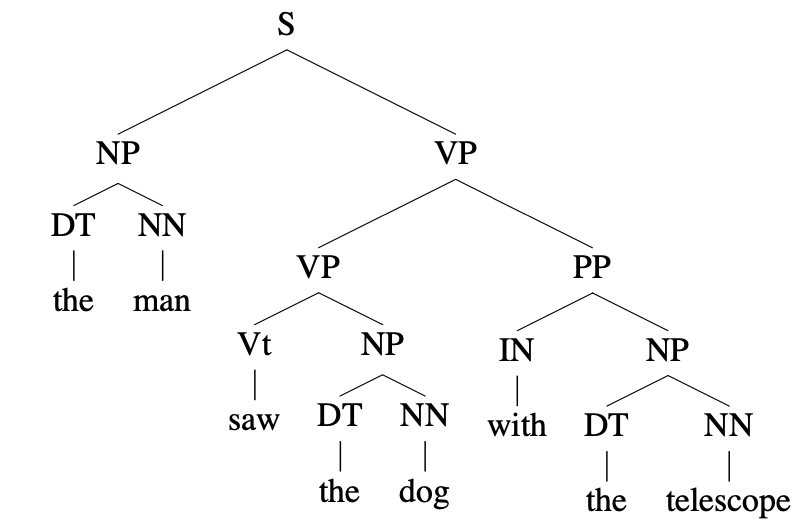
\includegraphics[height=4cm]{figures/parse-2.png}
    \end{figure}
    \vspace{-1em}
    What are the variables when constructing a tree rooted at $A$ spanning $x_i,\ldots,x_j$?\\
    \begin{itemize}
        \item The production rule $A\rightarrow B C$
        \item The splitting point $s$: $B$ spans $x_i,\ldots,x_s$ and
            $C$ spans $x_{s+1}, \ldots, x_j$
    \end{itemize}
\end{frame}

\begin{frame}
    {Bottom-up parsing}
    \begin{figure}
        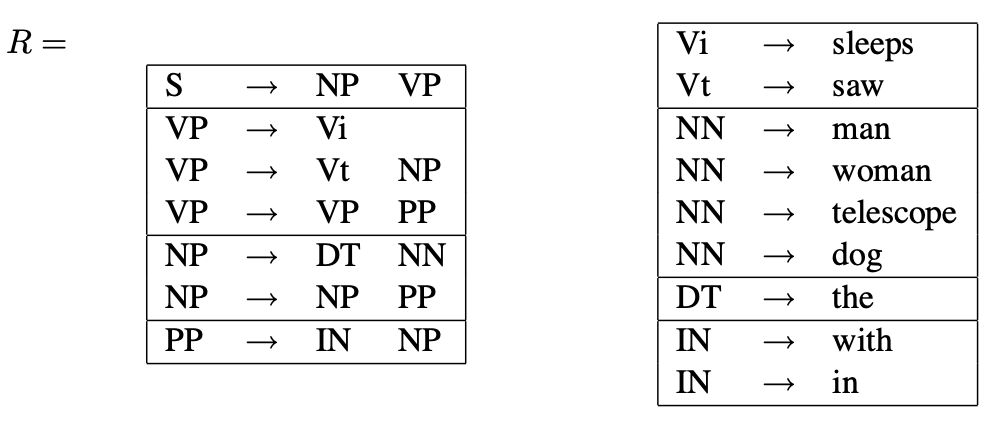
\includegraphics[height=3cm]{figures/toy-cfg-2.png}
    \end{figure}
    \vspace{14em}
\end{frame}

\begin{frame}
    {The CYK algorithm}
    Notation: $\sT(i,j,X)$ is the set of trees with root node $X$ spanning $x_i,\ldots,x_j$ 

    Subproblem:
    $$\pi(i,j,X) = \max_{t\in\sT(i,j,X)} p(t)$$

    Base case:
    $$
    \pi(i,i,X) = \begin{cases}
        q(X\rightarrow x_i) & \text{if } X\rightarrow x_i \in R \\
        0 & \text{otherwise}
    \end{cases}
    $$

    Recursion:
    $$
    \pi(i,j,X) = \max_{\substack{Y,Z \in N\\ s\in\pc{i,\ldots,j-1}}}
    q(X\rightarrow YZ)\times \pi(i,s,Y) \times \pi(s+1, j)
    $$

    Use backtracking to find the argmax tree.
\end{frame}

\begin{frame}
    {Variants of CYK}
    \textbf{Argmax}: find the most likely tree (analogous to Viterbi).
    $$
    \pi(i,j,X) = {\color{blue}\max}_{\substack{Y,Z\in N\\ s\in\pc{i,\ldots,j-1}}}
    q\p{X\rightarrow YZ} {\color{red}\times} \pi(i,s,Y) {\color{red}\times} \pi(s+1, j)
    $$

    \textbf{Recognition}: does the string belong to the language?
    $$
    \pi(i,j,X) = {\color{blue}\vee}_{\substack{Y,Z\in N\\ s\in\pc{i,\ldots,j-1}}}
    \1\pb{X\rightarrow YZ\in R} {\color{red}\wedge} \pi(i,s,Y) {\color{red}\wedge} \pi(s+1, j)
    $$

    \textbf{Marginalization}: what's the probability of the string being generated from the grammar? (the \textbf{inside algorithm})
    $$
    \pi(i,j,X) = {\color{blue}\sum}_{\substack{Y,Z\in N\\ s\in\pc{i,\ldots,j-1}}}
    q\p{X\rightarrow YZ} {\color{red}\times} \pi(i,s,Y) {\color{red}\times} \pi(s+1, j)
    $$

    Complexity?
\end{frame}

\begin{frame}
    {Summary}
    \begin{table}
        \renewcommand{\arraystretch}{1.7}
        \begin{tabular}{p{3cm}p{2cm}p{2cm}p{2cm}}
            \toprule
            & NB & HMM & PCFG \\
            \midrule
            output structure & & & \\
            learning & & & \\
            decoding & & & \\
            marginalization & & & \\
            unsupervised learning & & & \\
            \bottomrule
        \end{tabular}
    \end{table}
\end{frame}

\section{Discriminative parsing}

\begin{frame}
    {CRF for trees}
    \emph{Input}: sequence of words $x=(x_1, \ldots, x_n)$\\
    \emph{Output}: parse tree $y\in\sT(x)$\\
    \emph{Model}: decompose by production rules 
    $$
    p(y\mid x;\theta) \propto \prod_{(r,s)} \psi(r, s\mid x; \theta)
    $$
    \vspace{-1em}
    \begin{itemize}
        \item $r$: production rule
        \item $s$: start, split, end indices of the rule $r$
    \end{itemize}
    
    \begin{tikzpicture}
        \node {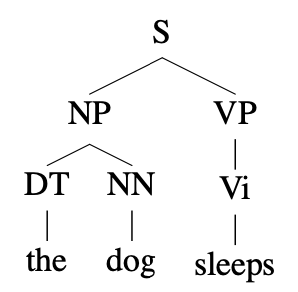
\includegraphics[width=3cm]{figures/toy-tree}};
    \end{tikzpicture}
\end{frame}

\begin{frame}
    {CRF parsing}
    Potential functions:
    \begin{align*}
        \psi(r, s\mid x; \theta) &= \exp\p{\theta\cdot\phi(r,s,x)}\\
        \prod_{(r,s)\in\sT(x)}\psi(r, s\mid x; \theta) &= \exp\p{\sum_{(r,s)\in\sT(x)}\theta\cdot\phi(r,s,x)}\\
    \end{align*}

    Learning: MLE\\
    \begin{enumerate}
        \item Compute the partition function by the inside algorithm
        \item Call autograd to compute the gradient (backpropagation)
    \end{enumerate}

    Inference: CYK
\end{frame}

\begin{frame}
    {Limitations of PCFG}
    \begin{figure}
        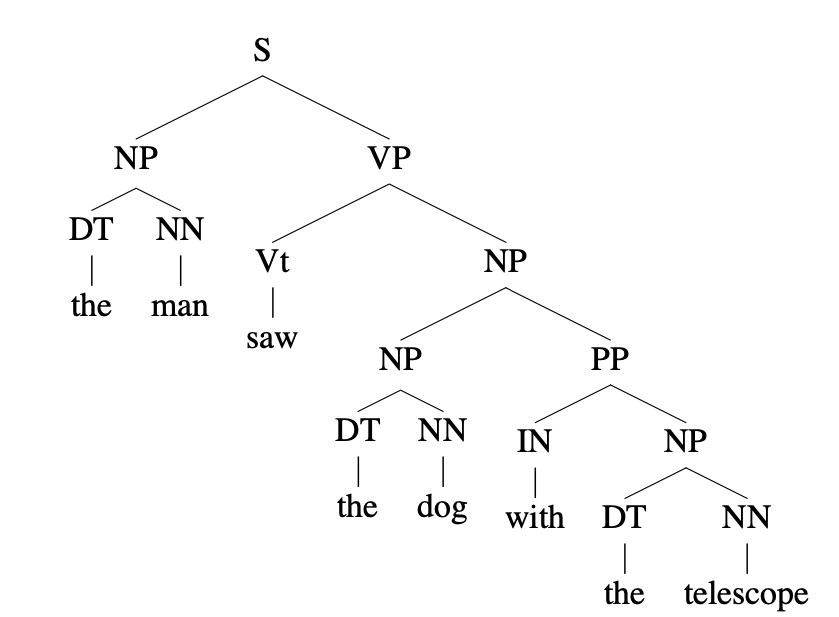
\includegraphics[height=5cm]{figures/parse-1}
    \end{figure}
    \pause
    No lexical information
\end{frame}

\begin{frame}
    {Lexicalized PCFG}
    Attach the ``head'' of the span to each non-terminal
    \begin{figure}
        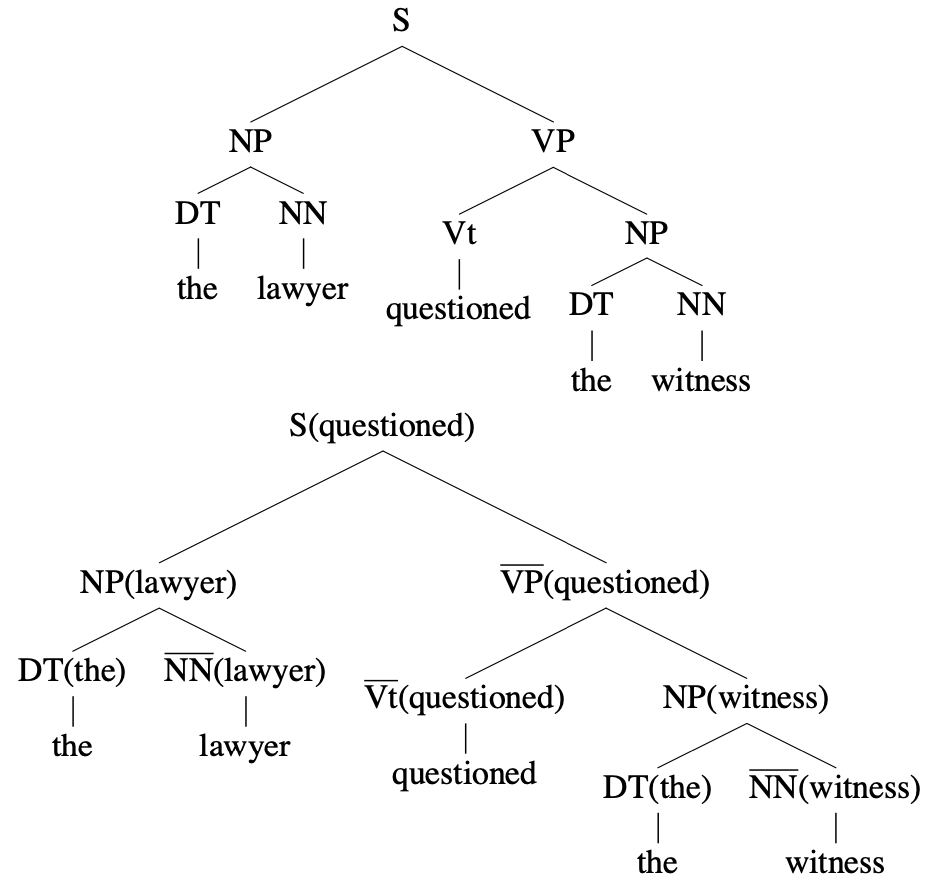
\includegraphics[height=7cm]{figures/lex-pcfg}
    \end{figure}
\end{frame}

\begin{frame}
    {Features}
    $$
    \text{local score} = \theta \cdot \phi(\text{VP $\rightarrow$ VBD NP}, (5, 6, 8), \text{...averted financial disaster...})
    $$
    \begin{figure}
        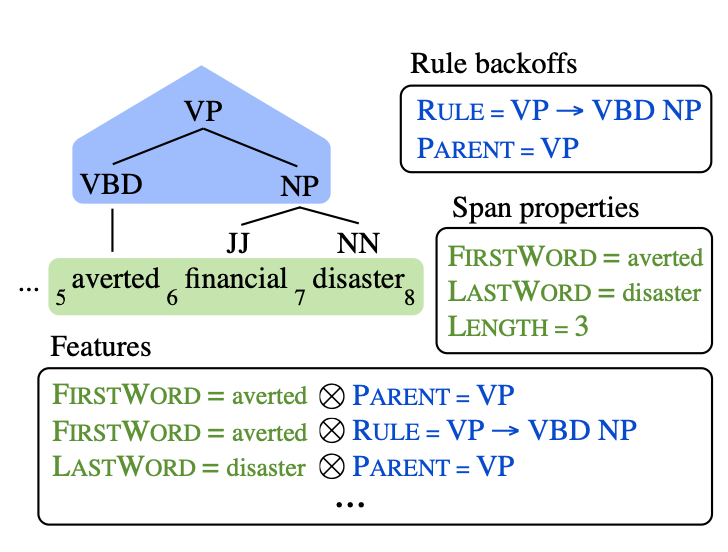
\includegraphics[height=5cm]{figures/parse-feature}
        \caption{Less grammar, more features. [Hall+ 14]}
    \end{figure}
\end{frame}

\begin{frame}
    {Neural CRF parser}
    \begin{figure}
        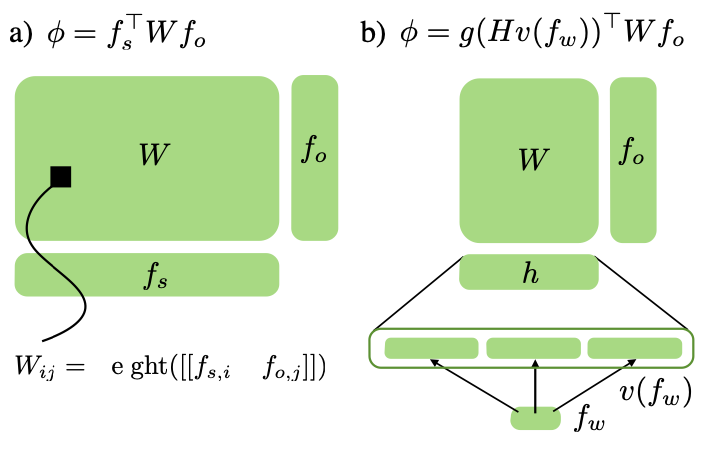
\includegraphics[height=5cm]{figures/neural-crf}
        \caption{Neural CRF Parsing. [Durrett+ 15]}
    \end{figure}
\end{frame}

\begin{frame}
    {Evaluation}
    \begin{align*}
        \text{recall} &= \frac{\# \text{correct constituents}}{\# \text{total constituents in gold trees}}\\\\
        \text{precision} &= \frac{\# \text{correct constituents}}{\# \text{total constituents in predicted trees}} \\\\
        \text{F1} &= \frac{2\times\text{precision}\times\text{recall}}{\text{precision}+\text{recall}}
    \end{align*}
    \begin{itemize}
        \item Labeled F1: the non-terminal node label must be correct
        \item Unlabeled F1: just consider the tree structure
    \end{itemize}
\end{frame}

\begin{frame}
    {Example}
    \begin{figure}
        \begin{subfigure}[b]{0.45\textwidth}
            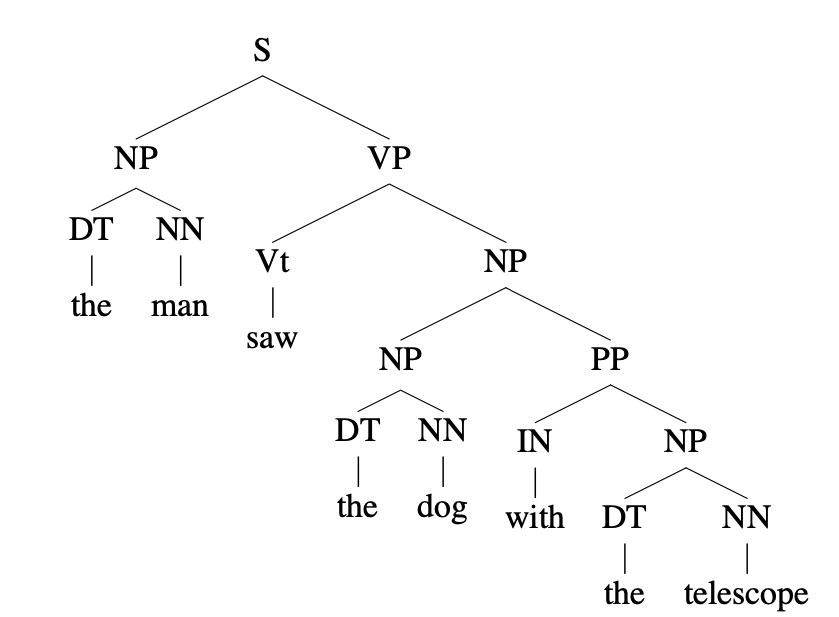
\includegraphics[width=\textwidth]{figures/parse-1.png}
            \subcaption{Gold.}
        \end{subfigure}
        \begin{subfigure}[b]{0.45\textwidth}
            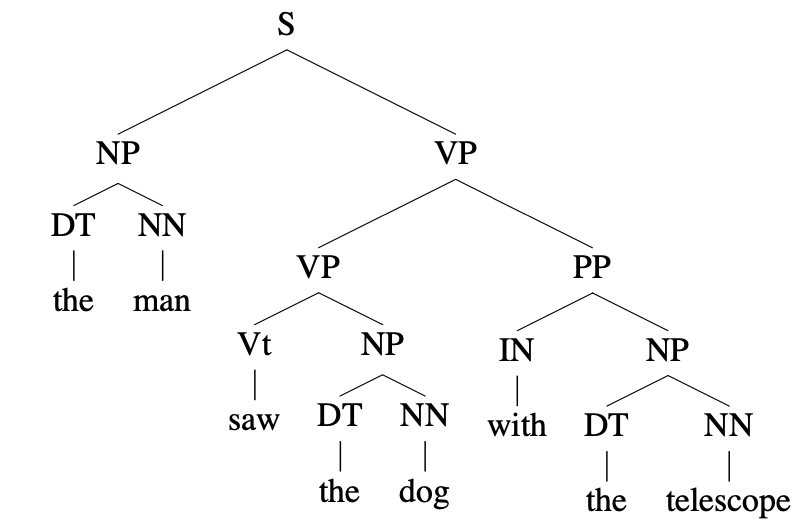
\includegraphics[width=\textwidth]{figures/parse-2.png}
            \subcaption{Predicted.}
        \end{subfigure}
    \end{figure}
\end{frame}

\end{document}
